\subsubsection{\stid{2.10} PROTEAS-TUNE - TAU Performance System}\label{subsubsect:tau}

\paragraph{Overview} 
The TAU Performance System is a versatile profiling and tracing toolkit that supports performance instrumentation, measurement, and analysis. It is a robust, portable, and scalable performance tool for use in parallel programs and systems over several technology generations. It is a ubiquitous performance tool suite for shared-memory and message-passing parallel applications written in C++, C, Fortran, Java, Python, UPC, and Chapel. In the PROTEAS project, TAU is being extended to support compiler-based instrumentation for the LLVM C, C++, and Fortran compilers using higher-level intermediate language representation. TAU is also targeting support for performance evaluation of directive based compilation solutions using OpenARC and it will support comprehensive performance evaluation of NVM based HPC systems.  Through these and other efforts, our objective to better support parallel runtime systems such as OpenMP, OpenACC, Kokkos, ROCm, and CUDA in TAU. Figure~\ref{figure:tau} gives an example of using TAU's parallel profile analysis tool, ParaProf.

\paragraph{Key Challenges} 
Scalable Heterogeneous Computing (SHC) platforms are gaining popularity, but it is becoming more and more complex to program these systems effectively and to evaluate their performance at scale. Performance engineering of applications must take into account multi-layered language and runtime systems, while mapping low-level actions to high-level programming abstractions.  Runtime systems such as Kokkos can shield the complexities of programming SHC systems from the programmers, but pose challenges to performance evaluation tools.  Better integration of performance technology is required.  Exposing parallelism to compilers using higher level constructs in the intermediate language provides additional opportunities for instrumentation and mapping of performance data.  It also makes possible developing new capabilities for observing multiple layers of memory hierarchy and I/O subsystems, especially for NVM-based HPC systems. 

\paragraph{Solution Strategy} Compilers and runtime systems can expose several opportunities for performance instrumentation tools such as TAU.  For instance, using the OpenACC profiling interface, TAU can tap into a wealth of information during kernel execution on accelerators as well measure data transfers between the host and devices. This can highlight when and where these data transfers occur and how long they last.  By implementing compiler-based instrumentation of LLVM compilers with TAU, it is possible to how the precise exclusive and inclusive duration of routines for programs written in C, C++, and Fortran.  Furthermore, we an take advantage of the Kokkos profiling interface to help map lower level performance data to higher level Kokkos constructs that are relevant to programmers. The instrumentation at the runtime system level can be achieved by transparently injecting the TAU Dynamic Shared Object (DSO) in the address space of the executing application. This requires no modification to the application source code or the executable. 

\begin{figure}[htb]
\centering
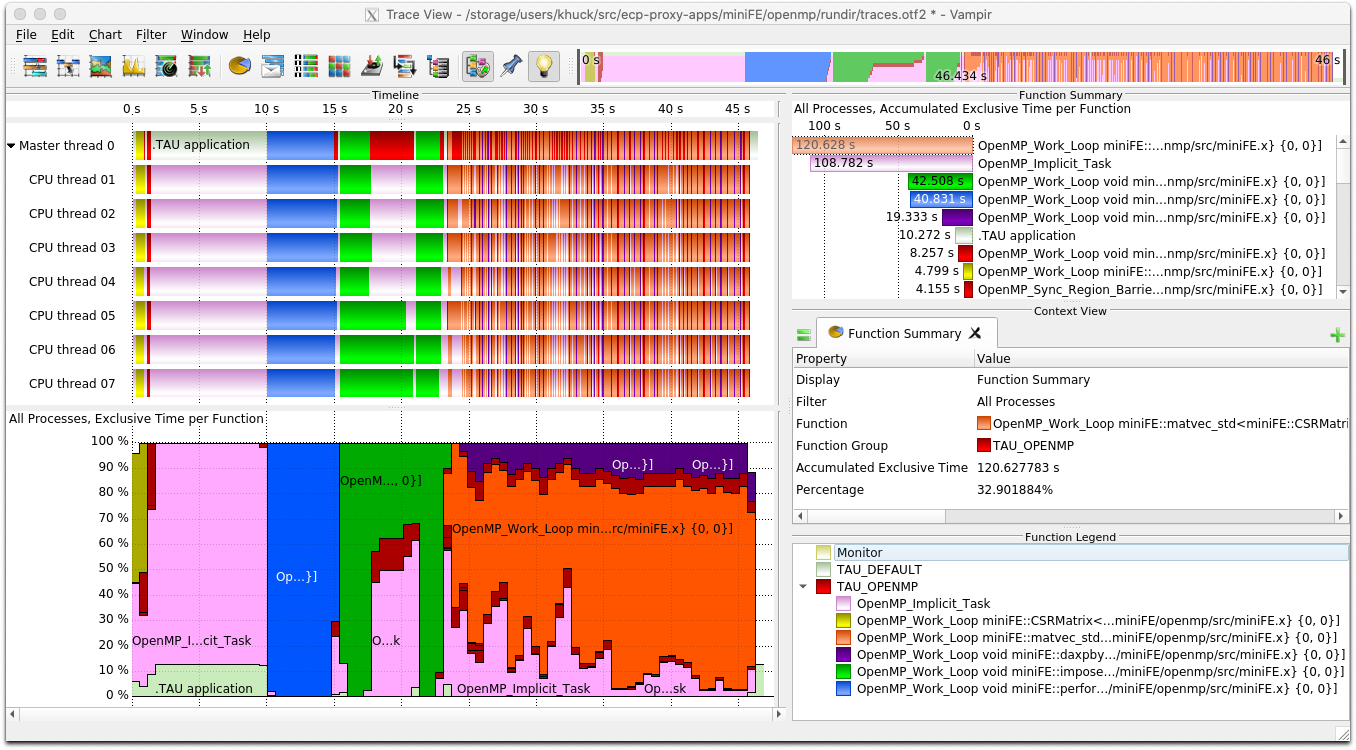
\includegraphics[width=6in]{projects/2.3.2-Tools/2.3.2.10-PROTEAS-YTUNE/miniFE_openmp_tau.png}
\caption{TAU was used to collect profiles and traces of ECP proxy applications like miniFE (trace shown in Vampir), observing OpenMP parallel regions, loops and synchronization without application instrumentation.}
\label{figure:tau:openmp}
\end{figure}

\begin{figure}[htb]
\centering
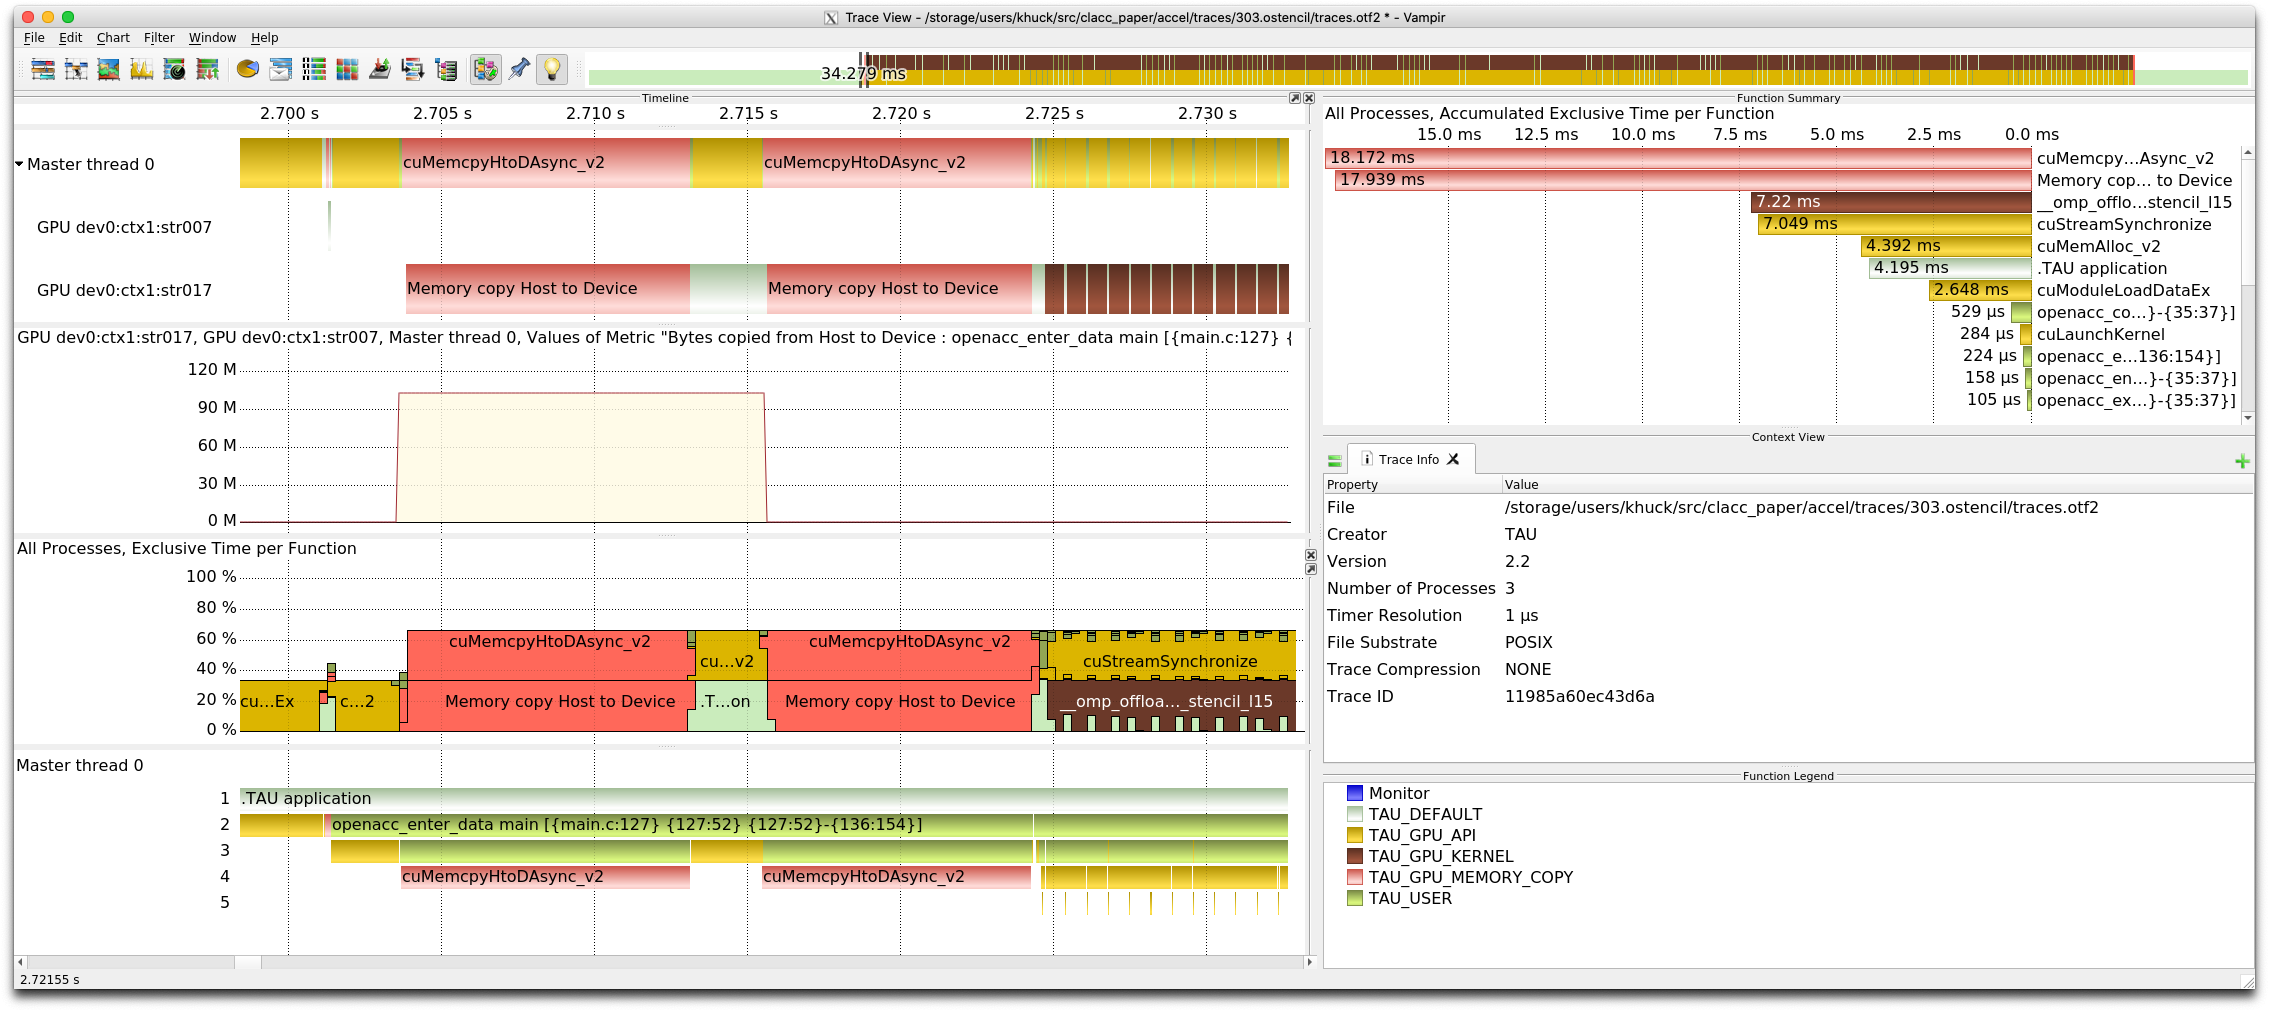
\includegraphics[width=6in]{projects/2.3.2-Tools/2.3.2.10-PROTEAS-YTUNE/clacc_tau.png}
\caption{TAU was used to collect profiles and traces of OpenACC benchmarks (303.stencil trace shown in Vampir), observing OpenACC regions and device offload events without application instrumentation.}
\label{figure:tau:clacc}
\end{figure}

\paragraph{Recent Progress}
\begin{enumerate}
\item \textbf{Updated CUDA support} Added preliminary support in TAU for NVIDIA A100 GPUs with support for CUDA 11.

\item \textbf{Updated OpenMP support} Updated OMPT support to OpenMP 5.0, tested with ECP Proxy applications miniFE and miniQMC as shown in the Vampir~\cite{vampir.eu} trace viewer in Figure~\ref{figure:tau:openmp}.

\item \textbf{Clacc support} Implemented/updated profiling support for OpenACC events provided by the Clacc compiler as shown in the Vampir trace viewer in Figure~\ref{figure:tau:clacc}.

\item \textbf{HIP} Added support for AMD GPUs with ROCm 3.3.

\item \textbf{CODAR} Updated TAU plugin for streaming profile and trace output to ADIOS2 for realtime application monitoring.  Integrated with Chimbuko framework for runtime trace analysis, demonstrated with XGC on Summit using 768 MPI ranks. (publication accepted to ISAV Workshop @SC20)

\item \textbf{E4S} Integrated TAU in E4S to support AMD GPUs. Both Docker and Singularity images posted on E4S.io website include TAU with support for NVIDIA and AMD GPUs.

\item \textbf{Kokkos} Updated support for Kokkos profiling interface in TAU (publication accepted to ProTools Workshop @SC20).

\item \textbf{LLVM Instrumentation} Implemented an LLVM module for selective instrumentation of C/C++ using TAU, tested with LLVM versions 6 through 12 and Clacc.

\item \textbf{CCAMP} Extended OpenACC and OpenMP interoperable framework, (publication to be presented at SC20).
\end{enumerate}

\paragraph{Next Steps}
\begin{enumerate}
\item \textbf{CUDA Enhancements} 
Implement new Profiling API and Perfworks Metrics API for CUDA/CUPTI 10+.

\item \textbf{OpenMP and OpenACC Enhancements} 
Explore and implement prototype measurement for OpenMP and OpenACC regions executed on target devices.

\item \textbf{New Architectures} 
We plan to support Intel OneAPI with Level Zero and the HPE Cray platform with AMD GPUs.

\item \textbf{Outreach}
Continued outreach activities to demonstrate comprehensive performance evaluation support in TAU for OpenARC, OpenACC, LLVM compiler-based instrumentation, CUDA, Kokkos, ROCm, and NVM based programming frameworks for SHC platforms. 

\item \textbf{E4S} 
Continued integration of TAU and PROTEAS-TUNE projects in the E4S. 

\item \textbf{LLVM Instrumentation} Add Fortran support for LLVM selective instrumentation module, add OpenACC profiling support for F18.

\item \textbf{TAU Instrumentation} Modernize TAU source-to-source auto-instrumentation support in TAU for C++ by replacing current parser front-end with LLVM based solution.

\end{enumerate}
